\begin{center}
    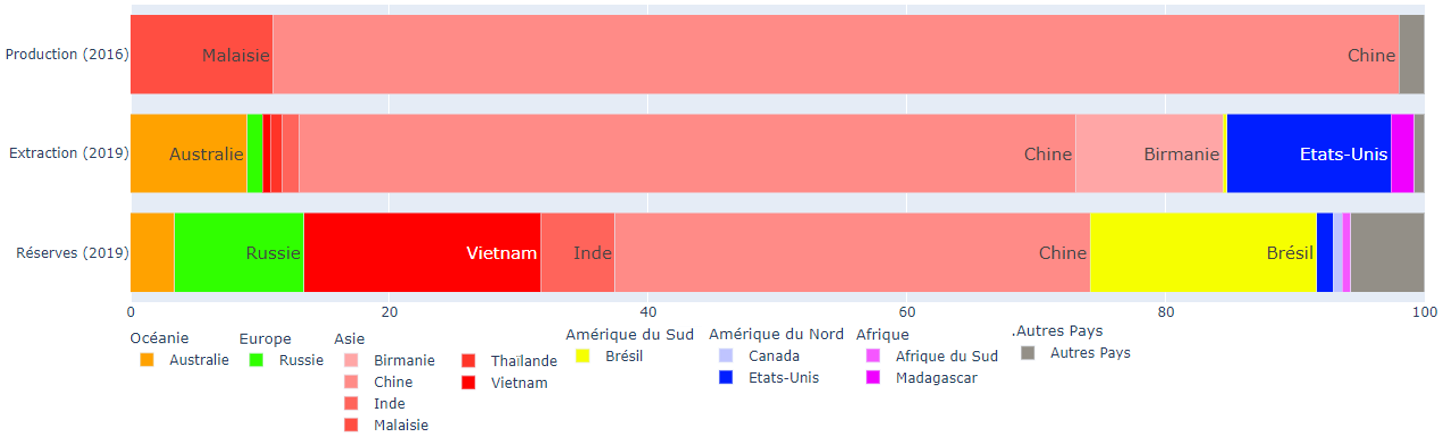
\includegraphics[width=\textwidth]{Illustration métaux/TR.png}
\end{center}
\begin{center}
    \textbf{Définition}
\end{center}
Les terres rares sont un groupe de métaux aux propriétés voisines comprenant le néodyme, le dysprosium, l'yttrium...\\

\begin{center}
    \textbf{Usages et consommation}
\end{center}
La demande en terres rares est particulièrement tirée par la fabrication
d'aimants permanents. Les aimants permanents sont fortement utilisés dans
le domaine de l'énergie pour la fabrication de génératrices (éoliennes en mer)
et de moteurs électriques (véhicules électriques).
\begin{center}
    \textbf{Prospective}
\end{center}
\begin{multicols}{2}
    \begin{center}
        \textit{Total RRE demand by sector and scenario}
    \end{center}
    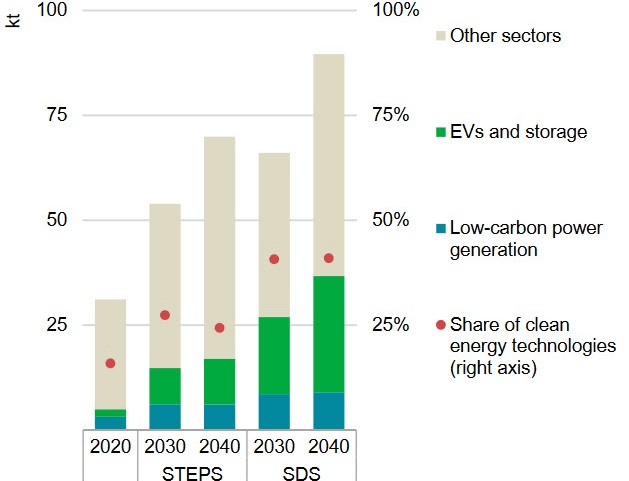
\includegraphics[width=0.45\textwidth]{Illustration métaux/RRE_prospective.jpg}
    \vfill\null
    \columnbreak
Il est prévu que la demande mondiale en terres rares augmente en partie à cause
de la décarbonation du mix énergétique mondial. La décarbonation du mix
énergétique mondial stimule la demande en majorité par le besoin en véhicule électrique
et sur un second plan par la construction de moyens de production bas-carbone.
Des projets miniers sont en développement sur tous les continents.
\end{multicols}
\begin{center}
    \textbf{Production et recyclage}
\end{center}
Le taux de croissance annuel moyen de la production minière de terres rares est entre 3 et 4\%. La production minière dépasse 150 kt/an. Le monopole de la Chine est en train de se réduire pour la production minière avec une production minière estimée à 57\% en 2020, contre plus de 95\% en 2011, grâce à de nouvelles productions en Birmanie ou aux Etats-Unis.
\begin{center}
    \textbf{Substituabilité}
\end{center}
Les terres rares ne peuvent pas être substituées sans pertes de performances
techniques pour la fabrication d'aimants permanents. 

\begin{center}
    \textbf{Prix}
\end{center}
Le prix des terres rares ont connu des épisodes de forte volatilité.
Le prix est d'environ 290 US\$/kg pour le dysprosium (2016) et et 50\$/kg pour le neodyme (2015).
\clearpage
\begin{center}
    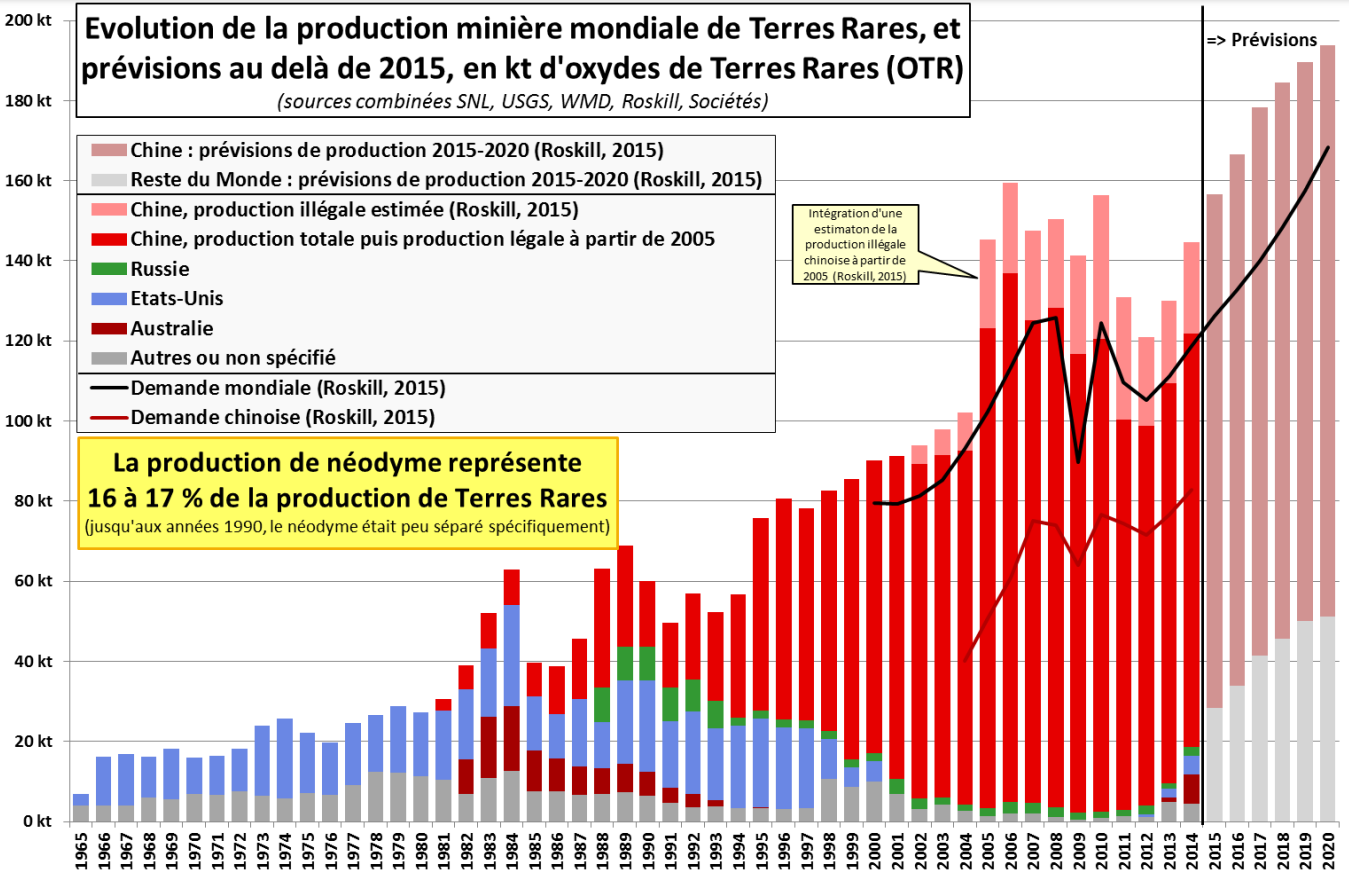
\includegraphics[width=12cm]{Illustration métaux/Dynamique_TR.png}
\end{center}
\begin{center}
    \textbf{Evènements géopolitiques}
\end{center}
La Chine a accéléré la limitation des exportations de terres rares en 2011 (voir encadré \hyperref[Chine]{\textit{Les terres rares chinoises : une arme  économique et géopolitique}})
\begin{multicols}{2}
    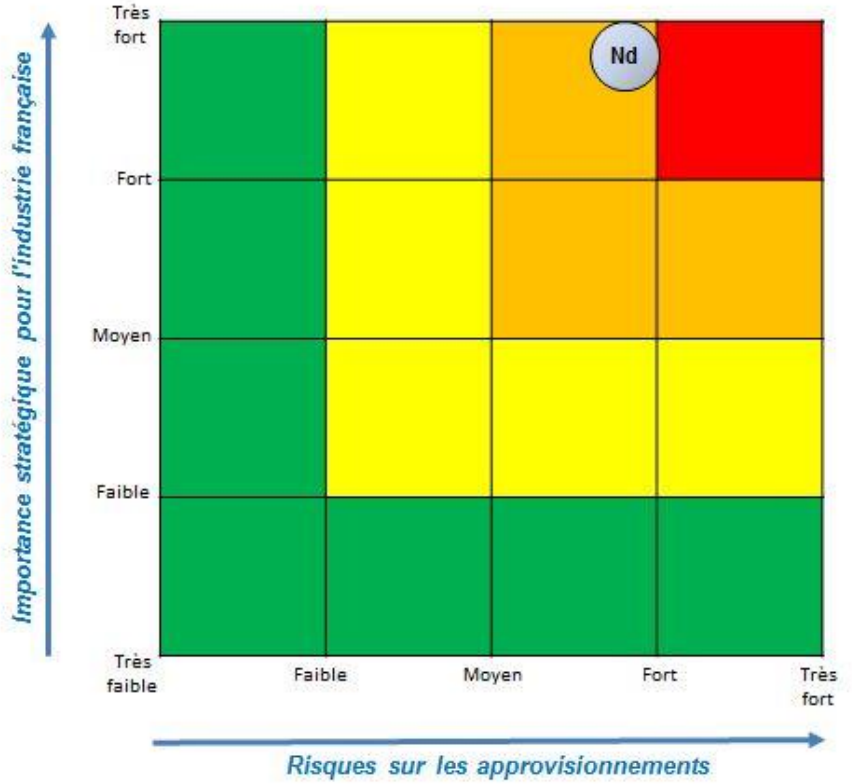
\includegraphics[width=0.35\textwidth]{Illustration métaux/TR_criticité.png}
    \begin{center}
    \textbf{Criticité en France}
    \end{center}
    Le risque sur les approvisionnements en terres rares est fort pour toutes les terres rares. Cependant l'impact stratégique sur l'industrie varie selon les terres rares. Pour le secteur énergétique, le néodyme est particulièrement stratégique pour la fabrication d'aimants permanents.
\end{multicols}
\begin{center}
    \textbf{Risques spécifiques}
\end{center}
Bien que la production minière se soit diversifiée, le raffinage reste dominé par la Chine. Il y a actuellement quatre unités de raffinage en dehors de Chine, en Malaisie, en Inde, en Estonie et en France.\\

\begin{center}
    \boxput*(0,1){
        \colorbox{white}{Terres rares en France}
    }{
    \setlength{\fboxsep}{15pt}
    \fbox{\begin{minipage}{14cm} 
    L'usine Solvay de La Rochelle a été fondée en 1948. A l’origine, le site fabriquait des pierres à briquets. Aujourd’hui, l’usine a une expertise reconnue dans la séparation et la purification des Terres Rares et la fabrication de produits de haute technologie servant les marchés de la dépollution automobile, de l’imagerie médicale et du polissage pour l’électronique et pour les verres de haute précision.\\
    Elle produit chaque année environ 4 000 tonnes de produits de formulation à base de terres rares pour les marchés de la catalyse, de la dépollution automobile, du polissage et de l’électronique (\cite{solvay_rochelle_2022})
    \end{minipage}}.
    }
\end{center}

